Arithmetic Logic Unit atau ALU adalah unit atau bagian CPU yang bertugas untuk
memproses kalkulasi-kalkulasi aritmatika dan operasi boolean/logika.

\begin{figure}[h]
    \centering
    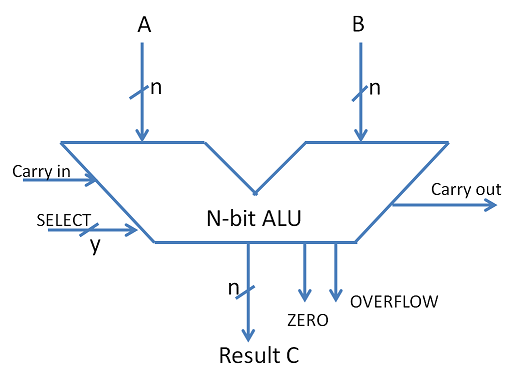
\includegraphics[scale=0.5]{ALUSYMBOLDIAG}
    \caption{Diagram Unit ALU}
    \label{fig:ALUSYMBOLDIAG}
\end{figure}


Menurut Ensiklopedia Brittanica, Arithmetic Logic Unit (ALU) adalah ``unit yang
berkaitan dengan empat fungsi aritmatika dasar, yaitu pertambahan, pengurangan,
perkalian, dan pembagian, serta operasi logika tertentu seperti perbandingan antara data
dan dalam memilih prosedur untuk menjawab suatu masalah atau bedasarkan kriteria yang
sudah ditentukan diawal``.

Secara struktural unit ini terdiri dari gerbang-gerbang logika semikonduktor
yang kemudian disusun hingga dapat memproses nilai-nilai integer biner.

Dalam memproses instruksi suatu ALU akan menerima dua input (A dan B),
ALU juga menerima sinyal operasi apa yang akan digunakan (SELECT),
akan mengeluarkan status yang dikirim ke register yang menyimpan
status akhir suatu operasi(Carry in, Carry out, Overflow dan Zero),
dan terakhir akan meng-output nilai dari kedua data atau angka yang telah dioperasikan.
